
\documentclass[aps,prl,twocolumn,eqsecnum,showpacs]{revtex4}
\usepackage{amssymb,amsmath}
\usepackage{bm, graphicx, amsmath}
\usepackage{bbm}
\usepackage[section]{placeins}


\usepackage[mathscr]{eucal}
\usepackage{graphicx}

\newcommand{\id}{{\mathbb I}}
\newcommand{\tr}{{\rm tr}\,}
\parskip=1em
  %%%%%%%%%%%%%%%%%%%%%%%%%%%%%%%%%%%%%%%%%%%%%%%%%%%%%%%%%%%%%%%%%%%%%%% %%%%%%%%%%%%%%%%%%%%%%%%%%%%%%%%%%%%%%%%%%%%%%%%%%%%%
 
 \newcommand{\abs}[1]{\left|{#1}\right|}
 \newcommand{\av}[1]{\left\langle #1 \right\rangle}
 
  \newcommand{\br}[1]{\langle #1|}
  \newcommand{\ke}[1]{|#1\rangle}
  \newcommand{\bk}[2]{\langle #1|#2\rangle}
  \newcommand{\kb}[2]{\ke{#1}\br{#2}}
  \newcommand{\var}[2]{\langle #1,#2\rangle} 
  
  \newcommand{\al}[1]{^{(#1)}}
  \newcommand{\da}{^\dagger} 
  
  \newcommand{\pt}[1]{\left( #1 \right)}
  \newcommand{\pq}[1]{\left[ #1 \right]}
  \newcommand{\pg}[1]{\left\{ #1 \right\}} 
  
  \newcommand{\lpt}[1]{\left( #1 \right.}
  \newcommand{\lpq}[1]{\left[ #1 \right.]}
  \newcommand{\lpg}[1]{\left\{ #1 \right.}
  \newcommand{\rpt}[1]{\left. #1 \right)}
  \newcommand{\rpq}[1]{\left. #1 \right]}
  \newcommand{\rpg}[1]{\left. #1 \right\}} 
  
  \newcommand{\pp}[2]{ {\mbox{\scriptsize$
  \begin{array}{c}
  #1\\
  #2
  \end{array}$} } }  
    \begin{document}

  \title{Probabilistically Perfect Cloning of Two Pure Qubit States}
  \author{authors}

  \affiliation{Department of Physics and Astronomy, Hunter College of the City University of New York, 695 Park Avenue, New York, NY 10065, USA}

  \begin{abstract}We solve the problem of making N perfect clones from M input copies of one of two pure states, for M$\geq$N and general a-priori probabilities.  The solution is a parametrized expression.  Geometrically it can be interpreted as when the line that represents the probability of failure is tangental to the unitarity constraint of the measurement process.
\end{abstract}
\pacs{03.67.-a, 03.65.Ta,42.50.-p }
\maketitle 

 The interest of quantum systems comes from their intrinsically probabilistic nature. If perfect cloning of quantum states were possible, this uncertainty would vanish, thus providing an intuitive argument for why perfect cloning is not determinstically feasible.  There have been two different strategies for dealing with the problem of cloning states:  one is to always produce clones that are 'as close' to the originals as possible, usually by means of global fidelity, as was first done for arbitrary states(cite Hillery) and then for one of two known pure states ( Bennett, etc).  

The other stategy is to sometimes make perfect copies, at the cost of sometimes failing to do so.  The seminal paper by Duan and Guo (cite Duan Guo) solved the problem of making perfect clones probabilistically for equal a-priori conditions, and set this success probability as an upper bound for general a-priori probabilities. While other work has improved on this bound ( ), there has until now been no general solution.  Other perfect probabilistic cloning schemes focus on other types of states ().

 Work has also been done on intermediate strategies where fidelity is maximized for a certain rate of failure, either pure states (cite Chefles) or mixed (Fiurasek, Setaski). There are practical reasons for wanting to produce perfect clones (cite applications), with applications in communication and computing. Experiments have been suggested (cite Fiurasek) and implemented (cite Muller) for cloning quantum states.

Finally, there is a deep relationship between cloning and state discrimination, where the asymptotic behavior of cloning strategies has been shown to reproduce known measurement results (cite Bae, Bennett). More information may be found in a review (cite review)

In this Letter, we provide an analytic solution to the general a-priori condition for the cloning of one of two pure qubits.  We provide arguments on why our choice of unitary conditions are optimal and then proceed to solve the problem by mapping the unitarity constraint to a parametrized space in which there is a clear geometric interpretation of the optimization process.

We begin by expressing the action of our desired unitary operator, $U$,  on one copy of our two input pure qubit states, $\ke {\psi_1}$ and $\ke {\psi_2}$.  The generalization to more input states is straightforward and will be addressed later in the letter. The most general expression of such a unitary is:
%
\begin{eqnarray}
U|\psi_1\rangle|0\rangle&=& \sqrt{p_1}|\Psi_1\rangle|\alpha_1\rangle +\sqrt q_1 |\Phi_1\rangle,\\
U|\psi_2\rangle|0\rangle&=& \sqrt{p_2}|\Psi_2\rangle|\alpha_2\rangle +\sqrt q_2 |\Phi_2\rangle.
\end{eqnarray}
%
Here we start with our ancilla in state $\ke 0$, $p_i$ and $q_i$ are the success and failure rates of cloning the $i'th$ state for $i = 1,2$.  The cloned states $\ke {\Psi_i}$, ancillas associated with successful cloning $\ke {\alpha_i}$, and failure states $\ke {\Phi_i}$ are completely general.  It has been shown to be possible to clone using an arbitrary ancilla state (cite Anirban Roy). 

Our only assumption thus far is that the successful clones and failure output are orthogonal, so $(\tr_{\!\!\mathscr L}\Phi_i)|\alpha_j\rangle=0$ for all $i,j$, where  $\mathscr L$ contains the sucess and failure subspaces. To make clones we need the ancillary Hilbert space $ \ke 0$ of dimension at least $2N+2$. One subspace to represent a successful transformation and an orthogonal one for the failed outcome.  Projection onto these dimensions will tell us if we've successfully made clones.  The other $2N$ dimensions are for the clones.  If the success outcomes of each state are not equal, ie  $\bk {\alpha_1}{\alpha_2}\neq 1$, or if the same is true for failure outcomes, then we need at least $2N +3$ dimensions.

If we take the product of the transpose of (1) with (2), we find the unitarity condition is
\begin{equation}
s=\sqrt{p_1 p_2} s' \alpha+\sqrt{q_1 q_2}\phi
\end{equation}
where
$$
s = \bk {\psi_1}{\psi_2}, \quad s'=\langle\Psi_1|\Psi_2\rangle,\quad \alpha=\langle\alpha_1|\alpha_2\rangle,\quad \phi=\langle\Phi_1|\Phi_2\rangle
$$
Similarly taking the inner product of each equation with its transpose gives normalized probabilities $p_i+q_i=1,\quad i=1,2.$

First we provide a heuristic argument on the optimal values of $\phi$.  If $\phi \neq 1$, then we could probabilistically determine whether we recieved $\ke{\psi_1}$ by unambiguously discriminating the $\ke {\phi_i}$.  This would allow us to sometimes be certain of the input state, when we can always prepare two copies of the state,  thereby increasing the overall success rate of the cloning strategy.

For the stronger argument of optimality, we can still choose $s,s'\ge0$, but different phases for $\alpha$ and $\phi$ lead to different unitarity conditions. Note, however, that we may choose them to be real, since only their real part are relevant to the unitarity condition. So, we take $ \Im\,\alpha=\Im\,\phi=0$. 
We can reasonably assume that $s>s'$, namely, that the posterior states are more distinguishable that the original ones.

To finish our analysis of $\alpha$ and $\phi$ we develop a useful paramatrized expressions for the success and failure rates $p_i$ and $q_i$. If we use the transformations $\sqrt{p_i} = \cos \theta_i$ for $0\leq \theta_i \leq \pi/2$ we can write
\begin{eqnarray}
x =&\cos(\theta_1+\theta_2)={1-(1+s^n)t\over s^{n-m}}, \\
y =& \cos (\theta_1 - \theta_2)={1-(1-s^n)t \over s^{n-m}}.
\end{eqnarray}
Using these transformations in the unitarity condition (3), then taking absolute values, we find that the overlap $s$ is bounded from above by the overlaps $\phi$ and $s' \abs{\alpha}$
$$
s\le\left|-{\phi-s'\alpha\over2}x\right|+\left|{\phi+s'\alpha\over2}y\right|\le\max\left\{\phi,s'|\alpha|\right\}
$$
So necessarily $s\le\phi$, since otherwise $s\le \max\{\phi,s'|\alpha|\}<\max\{s,s'|\alpha|\}=s$. Now, we show that optimality requires $\alpha>0$. Consider the two curves (resp., blue and red in the next figure),
$$
s=s'|\alpha| \sqrt{p_1p_2}+\sqrt{q_1q_2}\phi,\qquad s=-s'|\alpha| \sqrt{p_1p_2} +\sqrt{q_1q_2}\phi
$$
and the straight line 
$$
q_1=\xi_1 t,\quad q_2=\xi_2 t,\qquad \xi_1,\xi_2\ge0,\quad \xi_1^2+\xi_2^2=1
$$
\begin{figure}[h]
\centering
$%
\begin{array}{c}
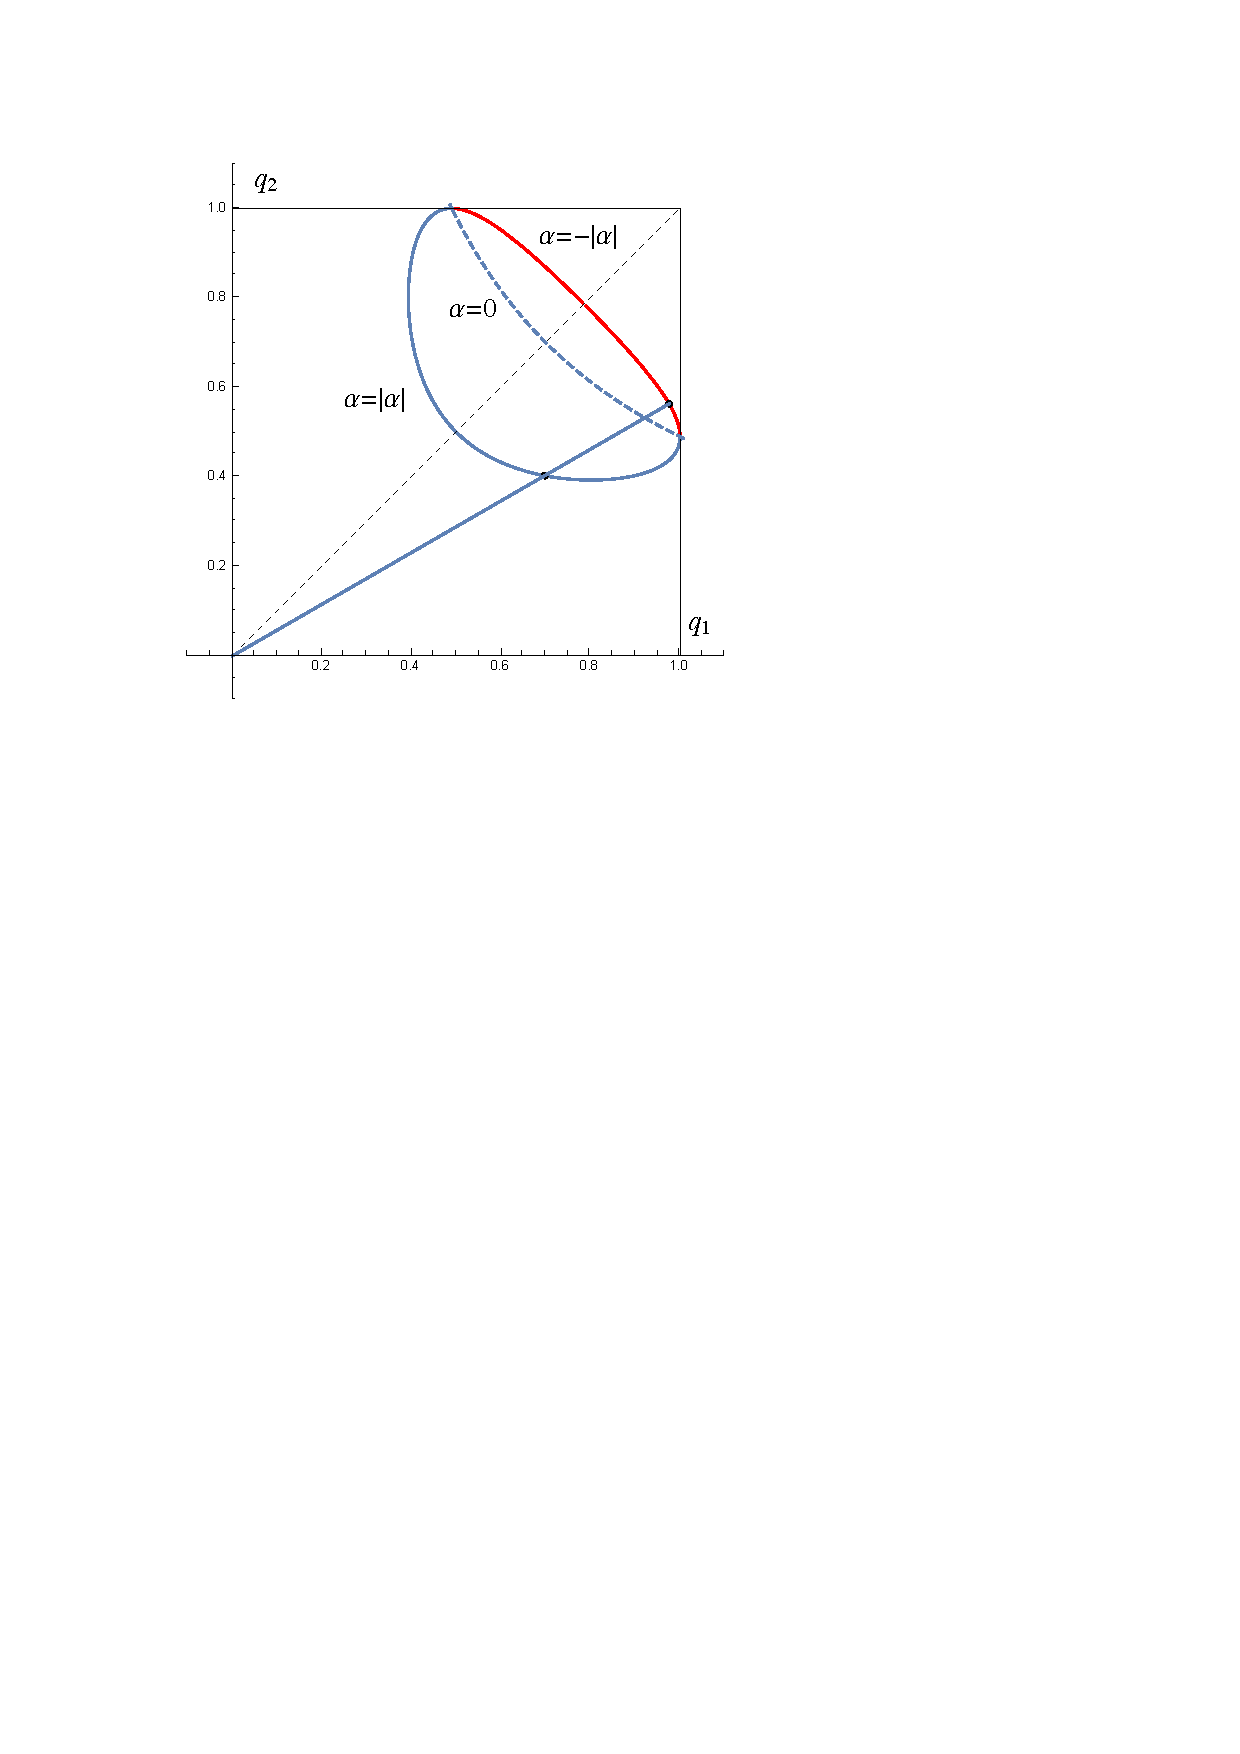
\includegraphics[width=23em]{Andi4_F3.pdf}\\
\end{array}%
$%
\caption{Unitarity curves for values of $\alpha$ positive, zero, and negative.}
\label{fig:Graphs}
\end{figure}

For given $\xi_1$, $\xi_2$, the distance from the origin to $(q_1,q_2)$ is~$t$. Substituting in the equations of the two curves we see from the resulting equation that whenever the straight line intersects the curve with negative $\alpha$ it also intersects the other. If $t_+$, $t_-$ give intersecting points for positive and negative $\alpha$ respectively, we have
$$
t_+\!=\!{s\!-\!|\alpha|s'\!\sqrt{1\!-\!\xi_1 t_+}\sqrt{1\!-\!\xi_2 t_+}\over\phi\sqrt{\xi_1\xi_2}}\le\!{s\over\phi\sqrt{\xi_1\xi_2}}$$
$$
t_- ={s\!+\!|\alpha|s'\!\sqrt{1\!-\!\xi_1 t_-}\sqrt{1\!-\!\xi_2 t_-}\over\phi\sqrt{\xi_1\xi_2}}\ge{s\over\phi\sqrt{\xi_1\xi_2}}
$$
Hence, the straight line $Q=\eta_1 q_1+\eta_2 q_2$ will intersect the curve with $\alpha=-|\alpha|$ for larger values of $Q$ than it will intersect that with $\alpha=|\alpha|$.
The limiting curve as $\alpha\to0$ is given by $t_0=s/(\phi\sqrt{\xi_1\xi_2})$. Therefore, it is the Unambiguous Discrimination hyperbola 
$$
q_1 q_2=(\xi_1t_0)(\xi_2 t_0)={s^2\over\phi^2}
$$
It is also clear from this picture that $t_+$ ($t_-$) is a decreasing (increasing) function of $|\alpha|$, Hence, the minimum value of $Q$ is given by $\alpha=1$, which implies that~$|\alpha_1\rangle=|\alpha_2\rangle$. Similarly, $\phi=1$, and hence $|\Phi_1\rangle=|\Phi_2\rangle$ is the optimal choice.

A convenient symmetric parametrization is
$$
x={1-(\phi+\alpha s')t\over \alpha s'/s};\qquad y={1-(\phi-\alpha s')t\over \alpha s'/s}
$$
The range of $t$ is given by the intersection of
$$
{1-\alpha s'/s\over\phi+\alpha s'}\le t\le{1+\alpha s'/s\over\phi+\alpha s'};\qquad
{1-\alpha s'/s\over\phi-\alpha s'}\le t\le{1\over\phi-\alpha s'};\qquad 
t\le{1\over\phi}
$$
We have
$$
{1-\alpha s'/s\over\phi-\alpha s'}\le t\le {1\over\phi}
$$

We return to the main problem having found the optimal values of the cloning rates from the unitarity conditions.  Now the equations for perfect probabilistic cloning $m\to n$, assuming $|\psi_1\rangle$, $|\psi_2\rangle$, as well as their prior probabilities $\eta_1$, $\eta_2$ are known, are 
\begin{equation}
U|\psi_i\rangle^m|0\rangle=\sqrt p_i |\psi_i\rangle^n|s\rangle+\sqrt q_i |f\rangle,\quad i=1,2,
\end{equation}
where $|s\rangle$ and $|f\rangle$ stand for success and failure, $\langle s| f\rangle=0$;  $|s\rangle$ is a rank 1 state, $\ke f$, the (garbage) state produced upon failure to clone, is of rank $n+1$, and $\ke 0$ and is of rank $n-m+1$.
Our optimal unitarity condition now reads as
$$
s^m=\sqrt{p_1p_2}s^n+\sqrt{q_1 q_2}, \quad n>m,
$$

Or using the substitutions for $x$ and $y$ as
\begin{equation}
s^m=-{1-s^n\over 2}x+{1+s^n\over2}y;\quad -1\le x\le1,\; 0\le y\le 1.
\end{equation}

. Hence, the allowed range of $t$ is~\footnote{The value $t=1$ is most easily found by inspection. For $t=1$, the argument of $\cos$ in the expression of $\sqrt p_1$ reads 
$$
{1\over2}\arccos(-s^m)+{1\over2}\arccos(s^m)={\pi\over2}
$$
for any value of $s^m>0$.
}
$$
{1-s^{n-m}\over 1-s^n}\le t\le  1.
$$

 where we use
\begin{eqnarray}
\sqrt q_1&=&\sin\left\{{1\over2}(\arccos{x}+\arccos{y})\right\},\\[1em]
\sqrt q_2&=&\sin\left\{{1\over2}(\arccos{x}-\arccos{y})\right\},
\end{eqnarray}
for
$$
{1-s^{n-m}\over 1-s^n}\le t\le \min\left\{{1\over1-s^n},{1+s^{n-m}\over1+s^n}\right\}.
$$

Finally, the region is manifestly symmetric under $p_1\leftrightarrow p_2$. Its shape, of course, is {\em independent} of the priors $\eta_1$ and $\eta_2$.  Figure 2 is an example for $m=1$, $n=2$:
\begin{figure}[h]
\centering
$%
\begin{array}{c}
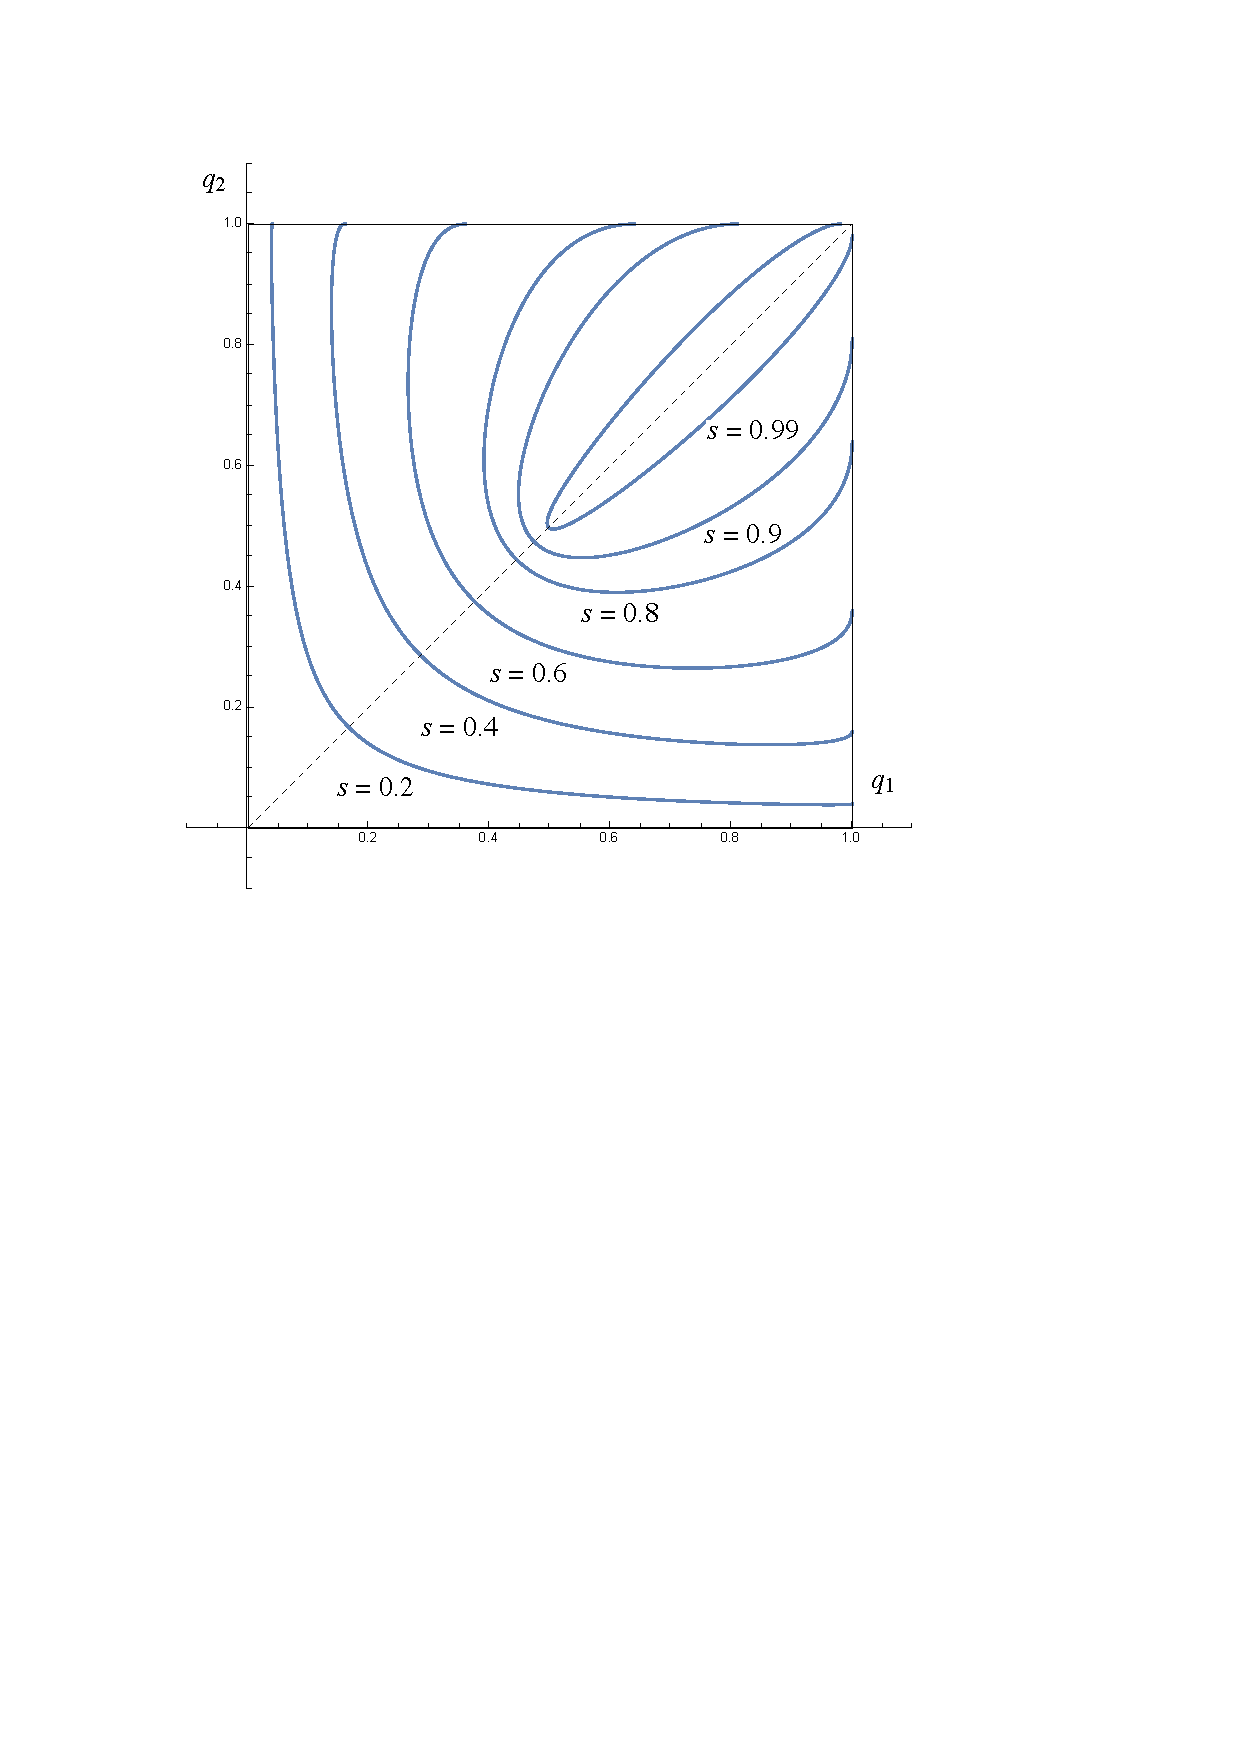
\includegraphics[width=23em]{Andi4_F1.pdf}\\
\end{array}%
$%
\caption{Unitarity curves for different values of the overlap $s$.}
\label{fig:Graphs}
\end{figure}
Note that we can easily get rid of the trigonometric functions and write
%
\begin{eqnarray*}
q_1&=&{1-xy+\sqrt{1-x^2}\sqrt{1-y^2}\over2},\\[.2em]
q_2&=&{1-xy-\sqrt{1-x^2}\sqrt{1-y^2}\over2}.
\end{eqnarray*}
%
For given values of initial conditions $\eta_1$ and $s$, we have one of the curves seen in Fig. 2 representing the unitarity constraint.  This curve represents the set of solutions for optimal $(q_1,q_2)$ for a given overlap.  Our goal is to find the particular solution for a given a-priori probability $\eta_1$.  

For this, we see in the same plane we see the class of lines with slope $-{\eta_1 \over \eta_2}$ representing the failure rate $Q=\eta_1 q_1+\eta_2 q_2 .$  It is convenient to represent this class using its normal vector, $\vec n=(\eta_1,\eta_2)$. From this set of admissable solutions, the minimum Q is the is the line in this class that intersects the unitarity curve once, and hence is tangent to it.  This tangency can also be represented by a normal vector, 
\begin{equation}
\vec t = ({-dq_2\over dt},{dq_1 \over dt})
\end{equation}
For optimality we know the two tangent vectors must be parallel: $\hat n = \hat t$.

We can express the line tangent to the unitary curve as $\eta_1 q'_1+\eta_2 q'_2=0$, where the primed variables are derivates with respect to $t$.  Using the constraint $1=\eta_1+\eta_2$ we have 
\begin{equation}
\eta_1={q'_2\over q'_2-q'_1},\quad \eta_2={q'_1\over q'_1-q'_2}.
\end{equation}
We could solve these equations for $t(\eta_1)$ and substitute into $q_1$ for the explicit expression if it were not a high order expression.  Numerically this is easily achieved.

\subsection{Minimization}

Our objective function is the average failure probability
$$
Q=\eta_1 q_1+\eta_2 q_2 .
$$
We view this as the equation of a straight line in the plane defined by $q_1$ and $q_2$ with normal vector $\vec n=(\eta_1,\eta_2)$. Since, $\eta_1$ and $\eta_2$ are probabilities, $\vec n$ belongs in the first quadrant. The minimum $Q$ is  that for which the corresponding straight line is tangent to the unitarity curve. Then
$$
\eta_1 q'_1+\eta_2 q'_2=0.
$$
Using that $1=\eta_1+\eta_2$ we have
$$
\eta_1={q'_2\over q'_2-q'_1},\quad \eta_2={q'_1\over q'_1-q'_2}.
$$
These equations define $\eta_1$ and $\eta_2$ in parametric form. 
Since the problem is symmetric under $1\leftrightarrow2$, it is sufficient to consider the range $0\le\eta_1\le 1/2$.
Then,
$$
0=\eta_1\;\Rightarrow\; q'_2=0\;\Rightarrow\; {d\over dt}\sqrt{q_2}=0
$$
gives the maximum value of $t$. We obtain
$$
0={d\over dt}\sqrt{q_2}={\sqrt p_2\over2s^{n-m}}\left({1+s^n\over\sqrt{1-x^2}}-{1-s^n\over\sqrt{1-y^2}}\right).
$$
Thus, the term in parenthesis must vanish. This gives
$$
t_{\rm max}={1-s^{2(n-m)}\over1-s^{2n}}<1.
$$
We also have the inequality,
$$
t_{\rm min}\equiv {1-s^{n-m}\over1-s^n}\le{1-s^{n-m}\over1-s^n}{1+s^{n-m}\over1+s^n}={1-s^{2(n-m)}\over1-s^{2n}}
=t_{\rm max} .
$$
Substituting back into $q_2$ we get that the minimum $q_2=Q$ is
$$
Q_{\rm min}=q_{2,{\rm min}}={s^{2m}-s^{2n}\over 1-s^{2n}}.
$$
The maximum value of $Q$ is at $t_{\rm min}$. Substituting in the expression of $Q$ we obtain
$$
Q_{\rm max}={s^m-s^n\over1-s^n}.
$$

For intermediate values of $t$,  $t_{\rm min}<t<t_{\rm max}$, we can plot the parametric curve given by
$$
(\eta_1,Q)=\left({q'_2\over q'_2-q'_1},{q'_2\over q'_2-q'_1}q_1+{q'_1\over q'_1-q'_2}q_2\right).
$$
One can check that
%
\begin{eqnarray*}
q'_1&=&{\sqrt{q_1(1-q_1)}\over s^{n-m}}\left({1+s^n\over\sqrt{1-x^2}}+{1-s^n\over\sqrt{1-y^2}}\right),\\[.25em]
q'_2&=&{\sqrt{q_2(1-q_2)}\over s^{n-m}}\left({1+s^n\over\sqrt{1-x^2}}-{1-s^n\over\sqrt{1-y^2}}\right).
\end{eqnarray*}
The next figure is a plot of $Q$ vs. $\eta_1$ for the same values of $s$ used in the previous figure.
$$
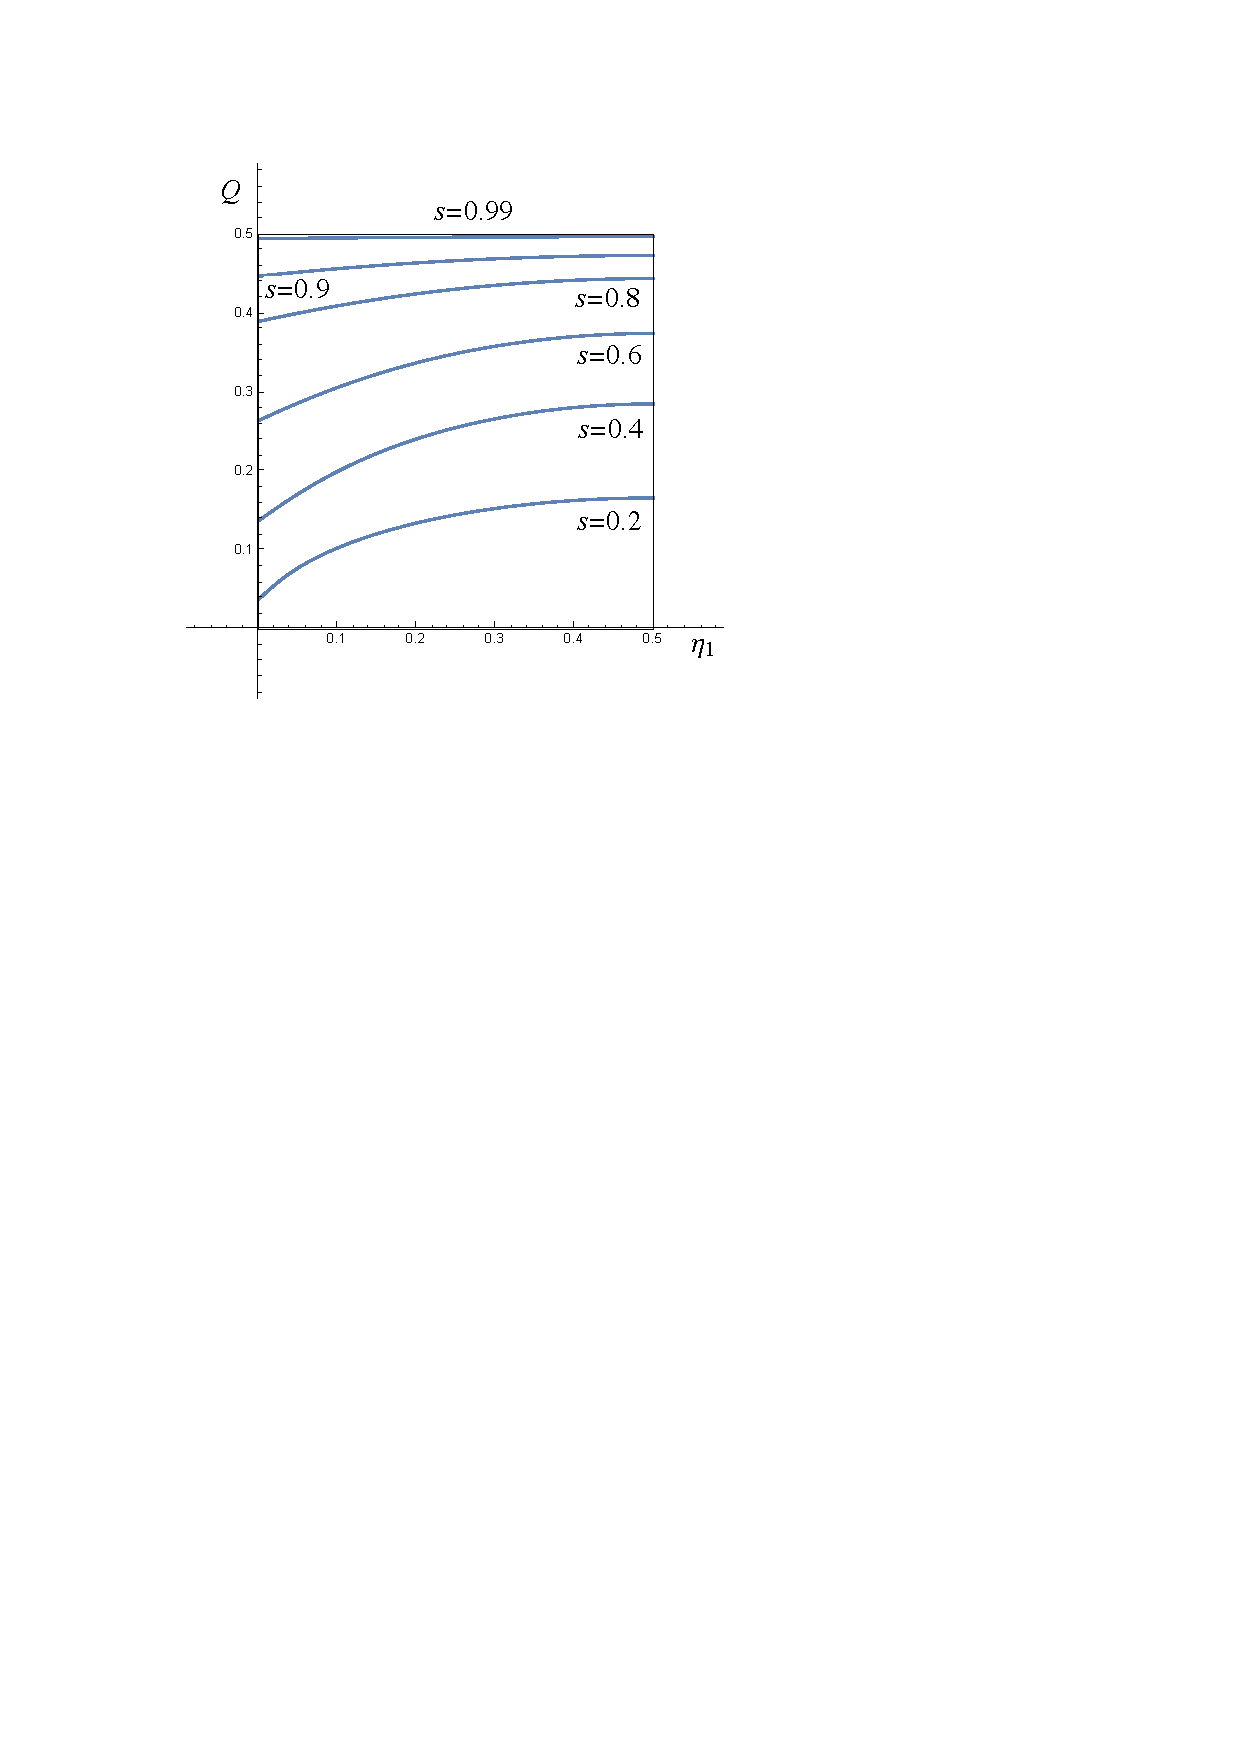
\includegraphics[width=22em]{Andi4_F2.pdf}
$$



  

\begin{thebibliography}{99}

\bibitem{Chefles} A. Chefles, Contemp. Phys. \textbf{41}, 401-424 (2000).

\bibitem{Bergou} Janos A. Bergou, J. Modern Optics \textbf{57}, 160-180 (2010)


\end{thebibliography}     
\end{document}
